\documentclass[10pt]{article}

\usepackage[english]{babel}
\usepackage[utf8x]{inputenc}
\usepackage{amsmath}
\usepackage{amssymb}
\usepackage{amsfonts}
\usepackage{graphicx}
\usepackage[ruled,linesnumbered,noend]{algorithm2e}
\usepackage{empheq}
\usepackage{float}
\usepackage{enumitem}
\usepackage{tikz}
\usepackage[colorlinks=true,urlcolor=blue]{hyperref}

\title{Introduction to Machine Learning, Fall 2014 - Exercise session III}
\author{Rodion ``rodde'' Efremov \\ 013593012}

\begin{document}
 \maketitle

\color{blue}
\section*{Problem 1 (3 points)}

\color{blue}
\section*{Problem 2 (3 points)}

\color{blue}
\section*{Problem 3 (3 points)}

\color{blue}
\section*{Problem 4 (15 points)}
In this exercise we implement an extremely simple prototype-based classifier to classify handwritten digits from the MNIST dataset, and compare that to a nearest-neighbor classifier.

\begin{itemize}
\item[(a)] Download the MNIST data from the course web page. In addition to the actual data, the package contains some functions for easily loading the data into Matlab/Octave/R and for displaying digits. See the README files for details. Load the first $N=5,000$ images using the provided function.

\color{black}
First we need to get to the directory containing the \texttt{loadmnist.m} file, run it, and load 5000 images along their class labels.
\begin{verbatim}
cd /path/to/mnist
run('loadmnist.m');
[X y] = loadmnist(5000);
\end{verbatim}
Now the matrix $X$ contains an image at each row (\texttt{X(i,:)} is the $i$th image).

\color{blue}
\item[(b)] Use the provided functions to plot a random sample of 100 handwritten digits, and show the associated labels. Verify that the labels match the digit images. (This is a sanity check that you have the data [is] in the right format.)

\color{black} As to verify the data, we need a randomly selected array of indices:
\begin{verbatim}
indices = randperm(5000, 100);
\end{verbatim}
After that we can draw the digits from the actual data and compare them to the actual labels:
\begin{verbatim}
visual(X(indices,:));
y(indices) # Prints the actual labels. 
           # Appeared to be in accord with the drawn digits.
\end{verbatim}

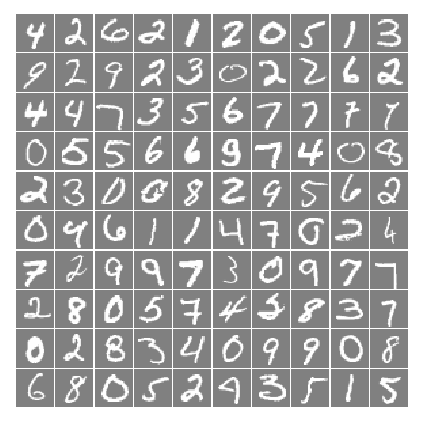
\includegraphics[width=\textwidth]{mnist_sample.png}

The first ten labels in vector \texttt{y} correspond to the digits in the upmost row:  4, 2, 6, 2, 1, 2, 0, 5, 1, 3, as expected.

\color{blue}
\item[(c)] Divide the data into two parts: A 'training set' consisting of the first 2,500 images (and associated labels), and a 'test set' containing the remaining 2,500 images (and their associated labels).

\color{black}
Dividing the data set is simple:
\begin{verbatim}
TrainingSet = X(1:2500,:);
TestSet = X(2501:5000,:);
TrainingSetY = y(1:2500);
TestSetY = y(2501:5000);
\end{verbatim}

\color{blue}
\item[(d)] For each ot the ten classes (digits 0-9), compute a class \textit{prototype} given by the mean of all the images in the training set that belong to this class. That is, select from the training set all images of class '0' and compute the mean image of these; this should look sort of like a zero. Do this for all ten classes, and plot the resulting images. Do they look like what you would expect?

\color{black}
First of all, we need a function to compute the prototypes:
\begin{verbatim}
function mean_vector = compute_prototype(T, labels, digit)
  mean_vector = zeros(1, size(T)(2));
  count = 0;
  for i = 1:size(T)(1)
    if labels(i) == digit
      mean_vector += T(i,:);
      count++;
    endif
  endfor
  mean_vector /= count;
endfunction
\end{verbatim}
Next, let us construct a $10 \times 784$-matrix $M$, whose rows are the prototypes. For all digits $d \in \{ 1, 2, \dots, 9 \}$, the prototype for $d$ is $M$'s $d$th row, and for the digit 0, the prototype is $M$'s 10th row.
\begin{verbatim}
function prototype_matrix = get_prototype_array(T, labels)
  prototype_matrix = zeros(10, 784);
  for i = 1:9
    prototype_matrix(i,:) = compute_prototype(T, labels, i);
  endfor
  prototype_matrix(10,:) = compute_prototype(T, labels, 0);
endfunction
\end{verbatim}

Now, running
\begin{verbatim}
visual(get_prototype_array(TrainingSet, TrainingSetY))
\end{verbatim}
we will obtain the following output:
\begin{figure}[H]
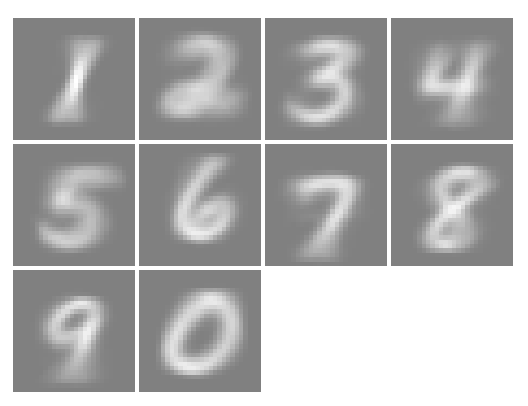
\includegraphics[width=\textwidth, keepaspectratio]{digit_prototypes.png}
\end{figure}
The prototypes look pretty good, but I suspect that 6 and 8 will be confused pretty often.

\color{blue}
\item[(e)] For each of the images in the test set, compute the Euclidian distance of the image to all 10 prototypes, and classify the test image into the class for which the distance to the distance to the prototype is the smallest. So, if a test image is closer to the prototype for '3' than it is to the prototypes for any of the other digits, predict its class to be '3'. Compute and display the resulting \textit{confusion matrix}.

\color{blue}
\item[(f)] Classify each of the test images with a nearest neighbor classifier: For each of the test images, compute its Euclidian distance to all (2,500) of the training images, and let the predicted class be the class of the closest training image. Compute and display the resulting confusion matrix.

\color{blue}
\item[(g)] Compute and compare the error rates of both classifiers (the prototype-based classifier and the nearest neighbor classifier). Which is working better? Based on the confusion matrix, which digits are confused with each other? Why do you think this is?
\end{itemize}

\end{document}